% #######################################
% ########### FILL THESE IN #############
% #######################################
\def\mytitle{IMPLEMENTATION OF BOOLEAN LOGIC IN ARDUINO IDE}
\def\mykeywords{}
\def\myauthor{B JAYASRI}
\def\contact{r180747@rguktrkv.ac.in}
\def\mymodule{}
% #######################################
% #### YOU DON'T NEED TO TOUCH BELOW ####
% #######################################
\documentclass[10pt, a4paper]{article}
\usepackage[a4paper,outer=1.5cm,inner=1.5cm,top=1.75cm,bottom=1.5cm]{geometry}
\twocolumn
\usepackage{graphicx}
\graphicspath{{./images/}}
%colour our links, remove weird boxes
\usepackage[colorlinks,linkcolor={black},citecolor={blue!80!black},urlcolor={blue!80!black}]{hyperref}
%Stop indentation on new paragraphs
\usepackage[parfill]{parskip}
%% Arial-like font
\usepackage{lmodern}
\renewcommand*\familydefault{\sfdefault}
%Napier logo top right
\usepackage{watermark}
%Lorem Ipusm dolor please don't leave any in you final report ;)
\usepackage{circuitikz}
\usetikzlibrary{calc}
\usepackage{tikz}

\usetikzlibrary{shapes, arrows, chains, decorations.markings,intersections,calc}
\usepackage{lipsum}
\usepackage{xcolor}
\usepackage{listings}
%give us the Capital H that we all know and love
\usepackage{float}
%tone down the line spacing after section titles
\usepackage{titlesec}
%Cool maths printing
\usepackage{amsmath}
\usepackage{tabularx}
%PseudoCode
\usepackage{algorithm2e}

\titlespacing{\subsection}{0pt}{\parskip}{-3pt}
\titlespacing{\subsubsection}{0pt}{\parskip}{-\parskip}
\titlespacing{\paragraph}{0pt}{\parskip}{\parskip}
\newcommand{\figuremacro}[5]{
    \begin{figure}[#1]
        \centering
        \includegraphics[width=#5\columnwidth]{#2}
        \caption[#3]{\textbf{#3}#4}
        \label{fig:#2}
    \end{figure}
}

\lstset{
frame=single, 
breaklines=true,
columns=fullflexible
}

\thiswatermark{\centering \put(-15,-100.0){
\includegraphics[scale=0.3]{logo}} }
\title{\mytitle}
  \author{\myauthor\hspace{1em}\\\contact\\FWC22159    IITH-Future Wireless Communications     Assignment-1\hspace{0.5em}\hspace{0.5em}\mymodule}
\date{}
\hypersetup{pdfauthor=\myauthor,pdftitle=\mytitle,pdfkeywords=\mykeywords}
\sloppy
% #######################################
% ########### START FROM HERE ###########
% #######################################
 
 \begin{document}
 \maketitle
     \tableofcontents 
    \begin{figure}[H]
        \centering
       \tikzset{every picture/.style={line width=0.75pt}} %set default line width to 0.75pt        

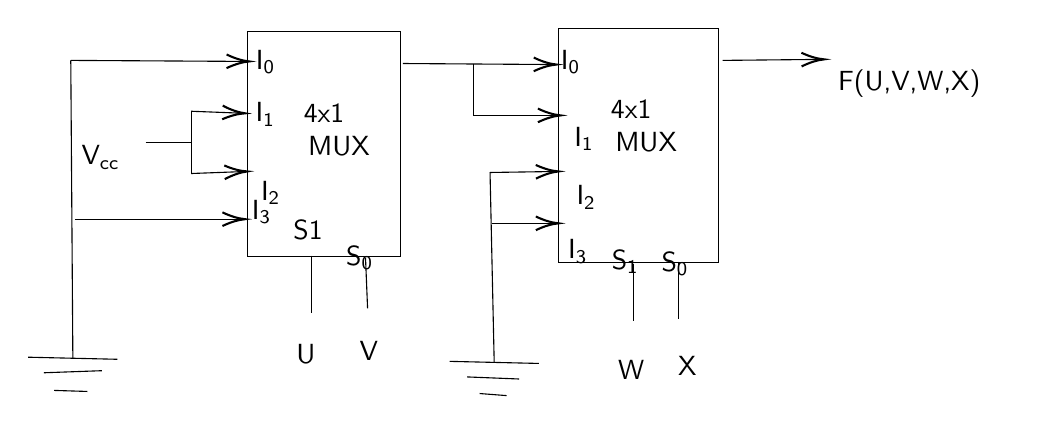
\begin{tikzpicture}[x=0.75pt,y=0.75pt,yscale=-1,xscale=1]
%uncomment if require: \path (0,391); %set diagram left start at 0, and has height of 391

%Shape: Rectangle [id:dp19533913691408] 
\draw   (160,54) -- (234,54) -- (234,162.5) -- (160,162.5) -- cycle ;
%Shape: Rectangle [id:dp7558719089146712] 
\draw   (310,52.5) -- (387,52.5) -- (387,165.5) -- (310,165.5) -- cycle ;
%Straight Lines [id:da6911766584504541] 
\draw    (235,69.5) -- (307,69.99) ;
\draw [shift={(309,70)}, rotate = 180.39] [color={rgb, 255:red, 0; green, 0; blue, 0 }  ][line width=0.75]    (10.93,-3.29) .. controls (6.95,-1.4) and (3.31,-0.3) .. (0,0) .. controls (3.31,0.3) and (6.95,1.4) .. (10.93,3.29)   ;
%Straight Lines [id:da45978453264104546] 
\draw    (269,69.5) -- (269,94.5) ;
%Straight Lines [id:da7820285564081373] 
\draw    (269,94.5) -- (309,94.5) ;
\draw [shift={(311,94.5)}, rotate = 180] [color={rgb, 255:red, 0; green, 0; blue, 0 }  ][line width=0.75]    (10.93,-3.29) .. controls (6.95,-1.4) and (3.31,-0.3) .. (0,0) .. controls (3.31,0.3) and (6.95,1.4) .. (10.93,3.29)   ;
%Straight Lines [id:da07769924779313142] 
\draw    (277,122) -- (308,121.53) ;
\draw [shift={(310,121.5)}, rotate = 179.13] [color={rgb, 255:red, 0; green, 0; blue, 0 }  ][line width=0.75]    (10.93,-3.29) .. controls (6.95,-1.4) and (3.31,-0.3) .. (0,0) .. controls (3.31,0.3) and (6.95,1.4) .. (10.93,3.29)   ;
%Straight Lines [id:da7950481680235839] 
\draw    (278,146.5) -- (308,146.5) ;
\draw [shift={(310,146.5)}, rotate = 180] [color={rgb, 255:red, 0; green, 0; blue, 0 }  ][line width=0.75]    (10.93,-3.29) .. controls (6.95,-1.4) and (3.31,-0.3) .. (0,0) .. controls (3.31,0.3) and (6.95,1.4) .. (10.93,3.29)   ;
%Straight Lines [id:da3899514607771639] 
\draw    (277,122) -- (279,213.5) ;
%Straight Lines [id:da7303317863785124] 
\draw    (191,162) -- (191,189.5) ;
%Straight Lines [id:da3818808743724176] 
\draw    (217,163) -- (218,187.5) ;
%Straight Lines [id:da8490459215964786] 
\draw    (346,166) -- (346,193.5) ;
%Straight Lines [id:da7079914024401793] 
\draw    (368,165) -- (368,192.5) ;
%Straight Lines [id:da7836237776539837] 
\draw    (75,68) -- (159,68.49) ;
\draw [shift={(161,68.5)}, rotate = 180.33] [color={rgb, 255:red, 0; green, 0; blue, 0 }  ][line width=0.75]    (10.93,-3.29) .. controls (6.95,-1.4) and (3.31,-0.3) .. (0,0) .. controls (3.31,0.3) and (6.95,1.4) .. (10.93,3.29)   ;
%Straight Lines [id:da707568149544794] 
\draw    (77,144.5) -- (157,144.5) ;
\draw [shift={(159,144.5)}, rotate = 180] [color={rgb, 255:red, 0; green, 0; blue, 0 }  ][line width=0.75]    (10.93,-3.29) .. controls (6.95,-1.4) and (3.31,-0.3) .. (0,0) .. controls (3.31,0.3) and (6.95,1.4) .. (10.93,3.29)   ;
%Straight Lines [id:da8308280317532427] 
\draw    (133,92.5) -- (157,93.42) ;
\draw [shift={(159,93.5)}, rotate = 182.2] [color={rgb, 255:red, 0; green, 0; blue, 0 }  ][line width=0.75]    (10.93,-3.29) .. controls (6.95,-1.4) and (3.31,-0.3) .. (0,0) .. controls (3.31,0.3) and (6.95,1.4) .. (10.93,3.29)   ;
%Straight Lines [id:da6352618461110756] 
\draw    (133,122.5) -- (158,121.57) ;
\draw [shift={(160,121.5)}, rotate = 177.88] [color={rgb, 255:red, 0; green, 0; blue, 0 }  ][line width=0.75]    (10.93,-3.29) .. controls (6.95,-1.4) and (3.31,-0.3) .. (0,0) .. controls (3.31,0.3) and (6.95,1.4) .. (10.93,3.29)   ;
%Straight Lines [id:da5274095094397975] 
\draw    (133,92.5) -- (133,122.5) ;
%Straight Lines [id:da21122265174810606] 
\draw    (75,68) -- (76,211.5) ;
%Straight Lines [id:da8643095047732517] 
\draw    (54.5,211) -- (97.5,212) ;
%Straight Lines [id:da230586889259341] 
\draw    (62,218.5) -- (90,217.5) ;
%Straight Lines [id:da11723337640914089] 
\draw    (67,227) -- (83,227.5) ;
%Straight Lines [id:da9666468322375824] 
\draw    (257.5,213) -- (300.5,214) ;
%Straight Lines [id:da6320877194548482] 
\draw    (266,220.5) -- (291,221.5) ;
%Straight Lines [id:da8062146503874882] 
\draw    (285,229.5) -- (272,228.5) ;
%Straight Lines [id:da7512505525646902] 
\draw    (111,107.5) -- (133,107.5) ;
%Straight Lines [id:da7205484797945809] 
\draw    (389,68) -- (436,67.52) ;
\draw [shift={(438,67.5)}, rotate = 179.42] [color={rgb, 255:red, 0; green, 0; blue, 0 }  ][line width=0.75]    (10.93,-3.29) .. controls (6.95,-1.4) and (3.31,-0.3) .. (0,0) .. controls (3.31,0.3) and (6.95,1.4) .. (10.93,3.29)   ;

% Text Node
\draw (154,62) node [anchor=north west][inner sep=0.75pt]   [align=left] { \ \ I\textsubscript{0}};
% Text Node
\draw (175,94) node   [align=left] {\begin{minipage}[lt]{16.32pt}\setlength\topsep{0pt}
I\textsubscript{1}
\end{minipage}};
% Text Node
\draw (212,132) node   [align=left] {\begin{minipage}[lt]{68pt}\setlength\topsep{0pt}
I\textsubscript{2}
\end{minipage}};
% Text Node
\draw (125.5,114.75) node   [align=left] {\begin{minipage}[lt]{68pt}\setlength\topsep{0pt}
V\textsubscript{cc}
\end{minipage}};
% Text Node
\draw (161,134) node [anchor=north west][inner sep=0.75pt]   [align=left] {I\textsubscript{3}};
% Text Node
\draw (186,88) node [anchor=north west][inner sep=0.75pt]   [align=left] {\begin{minipage}[lt]{25.39pt}\setlength\topsep{0pt}
4x1
\begin{center}
MUX
\end{center}

\end{minipage}};
% Text Node
\draw (334,86) node [anchor=north west][inner sep=0.75pt]   [align=left] {\begin{minipage}[lt]{25.39pt}\setlength\topsep{0pt}
4x1
\begin{center}
MUX
\end{center}

\end{minipage}};
% Text Node
\draw (253,163) node   [align=left] {\begin{minipage}[lt]{68pt}\setlength\topsep{0pt}
S\textsubscript{0}
\end{minipage}};
% Text Node
\draw (229,209.5) node   [align=left] {\begin{minipage}[lt]{68pt}\setlength\topsep{0pt}
U
\end{minipage}};
% Text Node
\draw (259.5,208) node   [align=left] {\begin{minipage}[lt]{68pt}\setlength\topsep{0pt}
V
\end{minipage}};
% Text Node
\draw (301,62) node [anchor=north west][inner sep=0.75pt]   [align=left] { \ \ I\textsubscript{0}};
% Text Node
\draw (363,106) node   [align=left] {\begin{minipage}[lt]{68pt}\setlength\topsep{0pt}
I\textsubscript{1}
\end{minipage}};
% Text Node
\draw (364,134) node   [align=left] {\begin{minipage}[lt]{68pt}\setlength\topsep{0pt}
I\textsubscript{2}
\end{minipage}};
% Text Node
\draw (360,160) node   [align=left] {\begin{minipage}[lt]{68pt}\setlength\topsep{0pt}
I\textsubscript{3}
\end{minipage}};
% Text Node
\draw (384,217) node   [align=left] {\begin{minipage}[lt]{68pt}\setlength\topsep{0pt}
W
\end{minipage}};
% Text Node
\draw (413,215) node   [align=left] {\begin{minipage}[lt]{68pt}\setlength\topsep{0pt}
X
\end{minipage}};
% Text Node
\draw (381,165) node   [align=left] {\begin{minipage}[lt]{68pt}\setlength\topsep{0pt}
S\textsubscript{1}
\end{minipage}};
% Text Node
\draw (405,166) node   [align=left] {\begin{minipage}[lt]{68pt}\setlength\topsep{0pt}
S\textsubscript{0}
\end{minipage}};
% Text Node
\draw (490,79) node   [align=left] {\begin{minipage}[lt]{68pt}\setlength\topsep{0pt}
F(U,V,W,X)
\end{minipage}};
% Text Node
\draw (181,144) node [anchor=north west][inner sep=0.75pt]   [align=left] {S1};


\end{tikzpicture}

        \caption{\textbf{The logic realised by the circuit shown in figure is}}
        \label{figs:fig:1}
    \end{figure}
  \textbf{}{\mykeywords}
 \section{Abstract}
 
      The objective of this manual is to show how to implement the Boolean function of a given  4x1 multiplexer :
      
      \begin{center}
      Y=(U'V+V'U).(W'X'+WX')
      \end{center}

\section{Introduction}
  
    \paragraph{Mutiplexer}
    is a combinational  logic circuit designed to switch one  of  the several  inputs lines through a single common output line by the application of a control signal.
      \\ The implementation of multiplexer takes three steps\\1.To get the truth table of multiplexer\\2.To get the Boolean equation using the truth table by using k map.\\
      \section{Components}
     
       \begin{tabularx}{0.35\textwidth} { 
  | >{\raggedright\arraybackslash}X 
  | >{\centering\arraybackslash}X 
  | >{\raggedleft\arraybackslash}X | }
\hline
\textbf{Component} &  \textbf{Value} & \textbf{Quantity}\\
\hline
Arduino UNO &  & 1 \\  
\hline
Bread board & - & 1 \\
\hline
Jumper wires & M-M & 8 \\
\hline
Led & - & 1\\
\hline
Resistor & 150ohms & 1\\
\hline
\end{tabularx}
\begin{center}
    
\end{center}
       \subsection{Arduino} \vspace{5mm}
      The Arduino uno has some ground pins, analog input pins A0-A3 and digital pins D1-D13 that can be used for both input as well as output. It also has two power pins that can generate 3.3V and 5V.In the following exercises, only the ground, 5V and digital pins will be used.
   \section{Introduction of 4x1 Multiplexer}
       \paragraph{ 4x1 Multiplexer } 
	    has four data inputs I3,I2,I1,I0 two selection lines S1,S0 and one output Y. The block diagram of 4x1 Multiplexer is shown in the following Figure-1. One of these 4 inputs will be connected to the output based on the combination of inputs present at these two selection lines.
  
 
       
       
  \section{Truth table for 4x1 multiplexer}
   \begin{tabularx}{0.4\textwidth} { 
  | >{\centering\arraybackslash}X 
  | >{\centering\arraybackslash}X 
  | >{\centering\arraybackslash}X | }
\hline
 \textbf{S1}& \textbf{S0} & \textbf{Y}\\
\hline
0 & 0 & I0 \\  
\hline
0&1&I1 \\ 
\hline
1&0&I2\\
\hline
1&1&I3\\
\hline
\end{tabularx}
\begin{center}
Truth Table for 4x1 Mux
\end{center}
\section{Boolean Equation}
	 By solving the given multiplexer circuit diagram we get the boolean eayuation as fallows : Y=(U'V+V'U).(W'X'+WX')
\section{Truth table for given multiplexercircuit diagram}
\begin{tabularx}{0.46\textwidth} { 
  | >{\centering\arraybackslash}X 
  | >{\centering\arraybackslash}X 
  | >{\centering\arraybackslash}X
  | >{\centering\arraybackslash}X 
  | >{\centering\arraybackslash}X | }
  \hline
 U & V & W & W  & Y\\
\hline
0 & 0 & 0 & 0 & 0 \\  
\hline
0 & 0 & 0 & 1 & 0 \\ 
\hline
0 & 0 & 1 & 0 & 0 \\
\hline
0 & 0 & 1 & 1 & 0 \\
\hline
0 & 1 & 0 & 0 & 1 \\  
\hline
0 & 1 & 0 & 1 & 0 \\ 
\hline
0 & 1 & 1 & 0 & 1 \\
\hline
0 & 1 & 1 & 1 & 0 \\
\hline
1 & 0 & 0 & 0 & 1 \\
\hline
1 & 0 & 0 & 1 & 0 \\
\hline
1 & 0 & 1 & 0 & 1 \\
\hline
1 & 0 & 1 & 1 & 0 \\
\hline
1 & 1 & 0 & 0 & 0 \\
\hline
1 & 1 & 0 & 1 & 0 \\
\hline
1 & 1 & 1 & 0 & 0 \\
\hline
1 & 1 & 1 & 1 & 0 \\
\hline
\end{tabularx}
\begin{center}
TABLE 1
\end{center}
\section{Hardware}
1. Connect Arduino to the computer and upload the code in to the arduino.Make 2,3,4,5 pins as input pins and 13 pin as output pin. Corresponds to the given inputs for the selection lines of multiplexer the outputs will be obtained at 13 pin. The builtin led in arduino is the indication of the output of multiplexer.
\section{Software}
 Download the following code
 \begin{lstlisting}
https://github.com/r180747/FWC-1/blob/main/Platformio/codes/main.cpp
 \end{lstlisting}
\end{document}

   
 

